\chapter{Writing/Using a library in C/C++}

\url{http://www.c-sharpcorner.com/Blogs/13113/how-to-know-dll-is-in-releasedebug-mode-in-vs-framework-2-0.aspx}


\section{Library dependencies}

All binary file(including an executable file, or a library file) rely upon the
existence of many libraries, which contain pre-written, presumably well-tested
subroutines that the programs can therefore simply "rely upon''.
In the Linux/Unix systems, you can easily have multiple versions of the same
library installed at the same time, i.e. each one is suffixed with the version
number, e.g. libstdc++.so.6.1, libstdc++.so.6.4. We can also have an alias, e.g.
\begin{verbatim}
libstdc++.so ---> libstdc++.so.6.1
\end{verbatim}
So, a programs can be very-generic or very-specific as to their requirements. 

The library files themselves also contain version-information so the linker can
be sure that the library-file it has found is compatible.
Once a library is built upon many different dynamically linked libraries, we
can check dependencies using \verb!ldd! tool (Sect.\ref{sec:ldd}).



References:
\begin{itemize}
\item
  \burl{http://www.yolinux.com/TUTORIALS/LibraryArchives-StaticAndDynamic.html} 
\end{itemize}

\section{Standard C library implementation}
\label{sec:standard-C-library}


To interact with devices (i.e. hardware), the Linux kernel implements a set of
standardized APIs, e.g. \verb!open()!, \verb!read()!.

However, we cannot directly make system calls in the same way that we call
normal functions because calls to the kernel aren't normal function calls, so they
can't be resolved by the linker. Instead, architecture-specific assembly
language thunks are used to call into the kernel - you can of course write these
directly in your own program too, but you don't need to because \verb!libc! (C
language - Sect.\ref{sec:libc}) or \verb!libstdc++! (C++ language -
Sect.\ref{sec:libstdc++}) provides them for you.

The order of execution-chain from a regular API, e.g. printf() is described
below, Fig.\ref{fig:API-call-chain}
{\tiny
\begin{verbatim}
call to printf()    -----> printf() in C library  -----> write() in the C
 library  ---> write() system call 
\end{verbatim}
}
\url{https://notes.shichao.io/lkd/ch5/}


\begin{figure}[hbt]
  \centerline{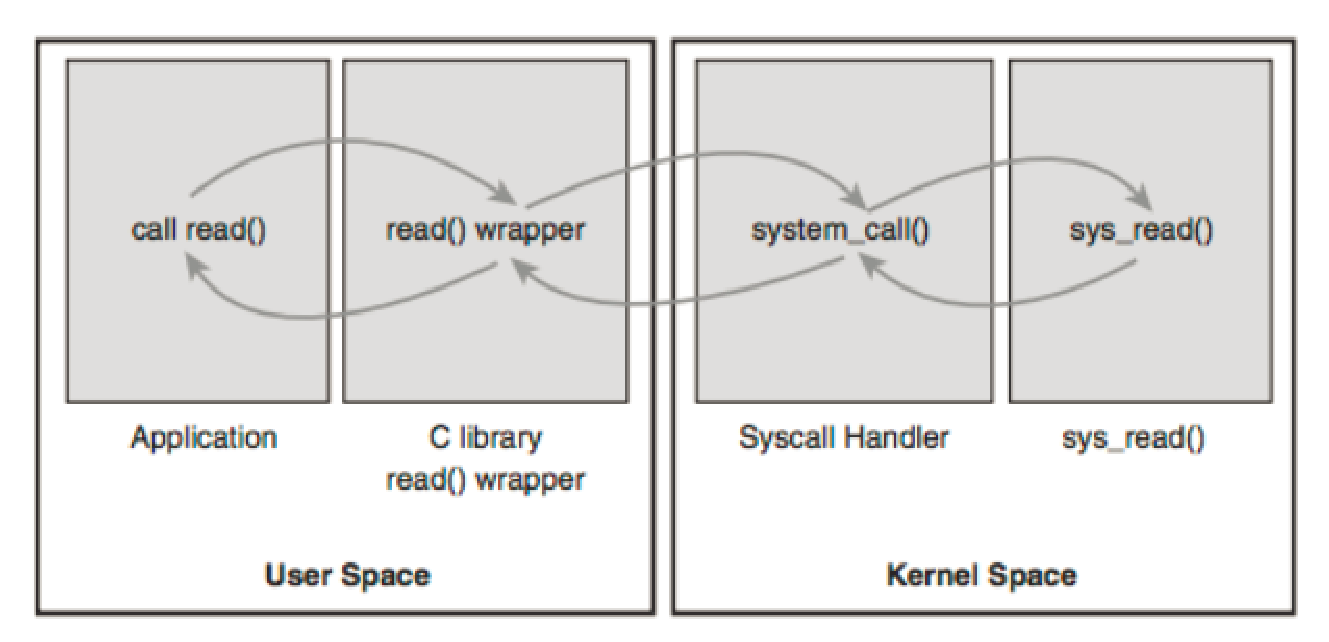
\includegraphics[height=3cm,
    angle=0]{./images/API-call-chain.eps}}
\caption{From a regular functional call to a system call}
\label{fig:API-call-chain}
\end{figure}


\subsection{-- glibc (libc)}
%\label{sec:glibc}

\verb!libc! (Sect.\ref{sec:libc}) is the early fork of glibc.
Later on, glibc is widely adopted (Sect.\ref{sec:glibc}).

So libc is just one of the libraries provided by glibc - and there are other
alternate implementations of libc other than glibc.

Note that not all standard C functions are in libc - most math functions are in
\verb!libm! (Sect.\ref{sec:libm}).
However, the glibc (GNU libc) project provides more than just libc - it also
provides the libm mentioned earlier, and other core libraries like
\verb!libpthread!.

\subsection{-- CRT (Microsoft)}

Sect.\ref{sec:CRT}

\subsection{musl}
\label{sec:musl}

musl is a 'libc', an implementation of the standard library functionality
described in the ISO C and POSIX standards, plus common extensions, intended for
use on Linux-based systems.

\url{http://www.musl-libc.org/faq.html}

\section{Standard C++ library implementation}
\label{sec:standard-C++-library}
\label{sec:C++-standard-library}

A standard C++ library provides system-level APIS implemented based on C++
language standard for a certain operating system.
Most C++ standard libraries are implemented over the OS's C library
(Sect.\ref{sec:standard-C-library}).


\begin{itemize}
  
  \item libstdc++ (implementation for GNU g++ compiler - Sect.\ref{sec:GCC}):
  on GNU/Linux.

Linux components have been developed around GNU libstd++ for ages. Some of them
do not build on anything else.


  \item libc++ (implementation for clang++ compiler - Sect.\ref{sec:clang}): on
  Mac O/S
  
\begin{verbatim}
clang++ -stdlib=libc++
\end{verbatim}

While libc++ is strong in new features, it has some problems with legacy code.
\end{itemize}


Example:
The libstdc++ std::string is a different data structure than the libc++
std::string. The former is a reference counted design, whereas the latter is
not. Although they are API compatible, they are not ABI compatible. That means
that if you construct a std::string with libstdc++, and then pass it to other
code that is linked against libc++, the receiving code would think it has a
libc++ std::string.
To you the programmer the libstdc++ std::string and the libc++ std::string look
like the same type. But to the linker, they look like completely different types
(the clue is the \verb!std::__1! namespace). And the linker's view is correct.
They are completely different types.
\begin{verbatim}
  // libstdc++
std::string, required to be resolved against std::basic_string implementation.

  // libc++
std::string, required to be resolved against the std::__1::basic_string implementation
\end{verbatim}
\url{http://stackoverflow.com/questions/12542971/using-libstdc-compiled-libraries-with-clang-stdlib-libc}

The pre-C++11 gcc std::list is not ABI compatible with the C++11 spec of
std::list. So, libc++ is no more ABI incompatible
with pre-C++11 libstdc++ than a C++11-conforming libstdc++ will be.


\subsection{-- libc++ (LLVM)}
\label{sec:libc++}

\verb!libc++! is the standard C++ library implemented on Mac O/S (since
Marvericks), and being used by clang/clang++ compiler, as well as GCC 4.7+.
\begin{itemize}
  \item On OS X before Mavericks: libstdc++ (Sect.\ref{sec:libstdc++}) was the
  default.
\end{itemize}
Compile the code using libc++ library with \verb!-stdlib=libc++! flag, and 
\verb!-std=c++11! flag.

\begin{verbatim}
g++ -std=c++11 -stdlib=libc++ input.cxx -o a.out
g++ -std=gnu++11 -stdlib=libc++ input.cxx -o a.out
clang++ -std=c++11 -stdlib=libc++ input.cxx -o a.out
clang++ -std=gnu++11 -stdlib=libc++ input.cxx -o a.out
\end{verbatim}

NOTE: libc++ is a new implementation of the C++ standard library, targeting C++11
(Sect.\ref{sec:C++11}). libc++ is not 100\% complete on GNU/Linux, and there's
no real advantage to using it when libstdc++ is more complete.
\url{http://libcxx.llvm.org/docs/}



\subsection{-- libstdc++ (GNU)}
%\subsection{libstdc++ : standard C++ library}
\label{sec:libstdc++}

\verb!libstdc++! is the standard C++ library implemented for GNU C++ Compiler
(Sect.\ref{sec:GCC}).
\begin{itemize}
  \item libstdc++ version 5: mainly needed for older pre-compiled packages
  
  \item libstdc++ version 6:
\end{itemize}
As libstdc++ is tightly integrated with g++ compiler development,
development of libstdc++ tending to be tied fairly closely to the matching
version of g++.

On Linux: In general, all commonly available linux distributions will use
libstdc++ by default.

\begin{verbatim}
clang++ -std=c++11 input.cxx -o a.out
clang++ -std=gnu++11 input.cxx -o a.out
\end{verbatim}

libstdc++ 4.2 is the last version using GPL2 license.

libstdc++ 4.3+ uses GPL3 license.

\subsection{-- libstdcxx (Apache)}
\label{sec:libstdcxx}

It lacks C++11 supports, as it is discontinued, i.e. STDCXX 4.2.1 in May'08.

\subsection{-- STLport}

It lacks C++11 supports, as it is discontinued, i.e.
STLport 5.2.1 was released in Oct'08.

\subsection{-- C++RT (Windows)}

Sect.\ref{sec:C++_RT}.

\section{Write a static library}

\subsection{In Linux}

In C, we do
\begin{verbatim}
cc -Wall -c ctest1.c ctest2.c 

// static library
ar -cvq libctest.a ctest1.o ctest2.o

\end{verbatim}
then
\begin{verbatim}
// linking to executable
cc -o executable-name prog.c libctest.a

cc -o executable-name prog.c -L/path/to/library-directory -lctest
\end{verbatim}

\subsection{Visual Studio}

Create a static library using Visual Studio for C/C++ (Sect.)



\section{Write an DLL}

\subsection{In Linux}

For shared library, we do
\begin{verbatim}
gcc -Wall -fPIC -c *.c
gcc -shared -Wl,-soname,libctest.so.1 -o libctest.so.1.0   *.o
mv libctest.so.1.0 /opt/lib

// create the default version using symbolic link
ln -sf /opt/lib/libctest.so.1.0 /opt/lib/libctest.so
ln -sf /opt/lib/libctest.so.1.0 /opt/lib/libctest.so.1
\end{verbatim}

We use 
\begin{enumerate}
  \item \verb!-fPIC! to produce position-independent code, 

  \item  \verb!-shared! to produce a shared object (*.so) which can be linked with
  other objects to form an executable.

\end{enumerate}

Then
\begin{verbatim}
gcc -Wall -I/path/to/include-files -L/path/to/libraries prog.c -lctest -o prog

gcc -Wall -L/opt/lib prog.c -lctest -o prog

\end{verbatim}


%\subsection{Export DLL's APIs}
\subsection{In Windows (C/C++)}
\label{sec:__declspec(dllexport)}

Writing a DLL in Windows is similar writing code for a static .LIB in Windows,
except we need to explicitly specify which APIs are accessible from outside the
library.


Not all APIs defined in the DLL can be accessed by the code that link to the
DLL. You have two options:
\begin{enumerate}
  \item use a Microsoft specific identifier  \verb!__declspec(dllexport)! declaration in the function definition 
\url{https://msdn.microsoft.com/en-us/library/dabb5z75(VS.80).aspx}

  
Example: C++ code  
\begin{verbatim}
// header file
#ifndef ADD_H
#define ADD_H
int __declspec(dllexport) add(int a, int b);
#endif  // ADD_H
\end{verbatim}

and in the program that use the library 
\begin{verbatim}
#include "add.h"
int add(int a, int b) {
    return a + b;
}
\end{verbatim}
  
  \item
\end{enumerate}

Example: \verb!extern ``C''! is important with C code. 
\begin{verbatim}
#include <stdio.h>

extern "C"
{
  __declspec(dllexport) void DisplayHelloFromDLL()
  {
    printf ("Hello from DLL !\n");
  }
}
\end{verbatim}
\verb!__declspec(dllexport)! is a required prefix for all functions that we
want to make DLL functions available from an external application.


Example: 
\begin{verbatim}
#include <iostream>
#include "cuda.h"
#include "cuda_runtime.h"
#include "device_launch_parameters.h"

extern "C" __declspec(dllexport) int sumTEst(int a, int b)
{
    int c = 0;
    test<<<1,1>>>(a, b, &c);
    return c;
}
\end{verbatim}  

Now we can build and get a DLL.

In Visual Studio, we can create a DLL project
\begin{verbatim}
File/New Project (Ctrl-Shift-N)
   Visual C++ project
      Template: Win32 project
 
Name of Project: <DLL name>

Application Settings (Application Type): choose DLL
Check Empty Project 
\end{verbatim}
\url{http://www.codeproject.com/Articles/9826/How-to-create-a-DLL-library-in-C-and-then-use-it-w}

\begin{mdframed}

A shared library can be in 1 or 5 states when it comes to debug/release DLLs.
To investigate a DLL, in Windows, we can use \verb!ilDasm.exe! utility.

\begin{enumerate}
  \item A non-debugable DLL
  \item An optimized debug DLL
  \item An optimized release DLL
  \item A non-optimized debug DLL
  \item A non-optimized release DLL
\end{enumerate}

\end{mdframed}


Initially, one \verb!.cpp! file whose name the same name as the project; and
\verb!stdafx.cpp! file which is necessary (yet you don't need to edit it - Sect.\ref{sec:stdafx.h})
% To create a DLL project: 
% \begin{itemize}
%   \item File / New Project (Ctrl-Shift-N)
%   \item Visual C++ Templates: select win32 project
%   \item Application Settings: select DLL
% \end{itemize}


Add a new C++ source file, and enter functions. These functions can be exposed
as APIs or just for internal use. Those exposed as APIs can be called by other
codes that reference to this DLL.
Sect.\ref{sec:__declspec(dllexport)} describes how to expose an API.

Now, to build this code into DLL, we need to use \verb!/LD! option in Visual Studio (Sect.\ref{sec:building_DLL_/LD}).

\subsection{Entry point of DLL}

Every application, including library, needs entry point. It is the address that
is used to load in to CPU PC register. It's similar to an entrance in a
building. You can go everywhere on every of that 100 storeys and thousands of
offices but there is only one entrance. The entry point of a DLL is
\verb!__DllMainCRTStartup! for 32-bit DLL and \verb!_DllMainCRTStartup! for
64-bit DLL. The function calls \verb!DllMain()!, and if there is no
\verb!DllMain()!, the DLL will not be loaded.



A DLL can optionally specify an entry-point function. If present, the system
calls the entry-point function whenever a process or thread loads or unloads the
DLL. It can be used to perform simple initialization and cleanup tasks. For
example, it can set up thread local storage when a new thread is created, and
clean it up when the thread is terminated.

The \verb!DllMain! function is an optional entry point into a dynamic-link
library (DLL). However, as \verb!DllMain! is a placeholder for the
library-defined function name, you can define a different name as the entry
point using the \verb!/ENTRY:linker! option and name your entry-point function
something other than DllMain, the C run-time library will not get initialized
properly. Nevertheless, if you decide to write your own entry-point funciton, it
has to duplicate everything that \verb!_DllMainCRTStartup! does
(NOTE: 
.
When building DLLs in Visual C++, \verb!_DllMainCRTStartup! is linked in automatically
and you do not need to specify an entry-point function using the /ENTRY: linker
option.


Examples of entry point function:
\begin{verbatim}
int main() for consoles

WinMain() for Win32-GUI

DLLMain() for DLL's
\end{verbatim}
Sect.\ref{sec:without_main()} describes how use a different name for the entry-point in a console application.

IMPORTANT:  Don't call CreateProcess from DllMain, as it can create dead lock.
he standard way to get things done from DllMain is to create a thread to do the
work.
Calling functions that require DLLs other than Kernel32.dll may result in
problems that are difficult to diagnose.
For example, calling User, Shell, and COM functions can cause access violation
errors, because some functions load other system components.
 Conversely, calling functions such as these during termination can cause access
 violation errors because the corresponding component may already have been
 unloaded or uninitialized.

\section{Using a LIB in your project}

By default, all the symbols in a static library are visible to the linker and available for the linked program. 

Of course to compile your program you need the matching header (normally .h)
files of the static library. A static library has nothing to do with .def or
.exp files.

\section{Using a DLL in your project}

In order to compile an executable file (Sect.\ref{sec:executable_file}) using a
DLL, you need to tell the linker how the DLL can be used when linking.
The header file can only give some information, e.g. the function signature. But
the compiler still need to know the name of the DLL, and what symbols are
available in the DLL. This information can be stored in either
\begin{enumerate}
  \item an import library (Sect.\ref{sec:import_library})
  
The import library (.LIB) is automatically created when you compile a DLL file.
   
  \item a .exp file (export file): 
  
\end{enumerate}

We need both the header file and the binary files. 
\begin{itemize}
  \item Tell the compiler where to  look for your header files
  
  \item Tell the linker where to look for the library files (static or import
  libraries) 
  
There is no need to configure if dynamic library is used.
  
  \item \verb!#include! the header files in your program 
  
  \item (if dynamic libraries or import library is used) then make sure the
  location of the dynamic libraries can be found by the program at runtime.

The .dll file must be available when the executables run at run-time. 

\end{itemize}

In Visual Studio, read Sect.\ref{sec:VS_Configuration_Properties}

\subsection{Troubleshoot DLL version mismatch}

Many third-party uses C/C++ Runtime Library (Sect.\ref{sec:CRT},
Sect.\ref{sec:C++_RT}). However, this can cause a conflict issue when you use
one third-party DLL compiled using Visual Studio 2005, while the other
third-party DLL was compiled using Visual Studio 2008. Two versions of VS use
two different version of the CRT (Sect.\ref{sec:CRT}).

To know which CRT version was used to compile a DLL, we use \verb!DUMPBIN! tool (Sect.\ref{sec:dumpbin_command}). 
\begin{verbatim}
dumpbin /imports <dllname.dll>
\end{verbatim}
and search for MSVCRT**.dll, with \verb!**! will be the version number (70, 71, 80, 90). 


Suppose you are the third-party who develop the DLL. It is best to fix the same 
version of Runtime Library, regardless of which version of Visual Studio you use. 
This can be done by
\begin{enumerate}
  \item disable using default RunTime libraries
\begin{verbatim}
Project Properties->Linker->Input->Ignore All Default Libraries->Yes
\end{verbatim}

  \item create a custom library and link that to the project
\url{https://msdn.microsoft.com/en-US/library/k9a8ehy3(v=VS.80).aspx}
  
Microsoft VS allows you to compile your own version of CRT.
\begin{itemize}
  \item Run the Visual Studio Command Line tool as Administrator
  
  \item type
\begin{verbatim}
set vctools=C:\Program files\Microsoft Visual Studio x.x\VC
\end{verbatim}
with \verb!x.x! is the version of the Visual Studio.

  \item type
\begin{verbatim}
crt\src\bldnt.cmd
\end{verbatim}

This will run for a minute or so, compiling all the necessary libraries for your system, which returns
\begin{verbatim}
libcmt.lib
libcpmt.lib
_sample_.dll
_sample_.lib
\end{verbatim}
NOTE: \verb!_sample_.*! are the actually copies of msvcrXX.dll (where XX is your VS version). 
They are renamed so that they do not conflict with the actual MS libraries.


\end{itemize}

To compile a custom version of CRT that you can pack with your library.

\begin{verbatim}
'Additional Dependencies=.\_sample_lib'
\end{verbatim}
  
The other alternative is just to ignore the default CRT libraries by going to
'Ignore Specific Library=msvcr9.0.lib' and place
\begin{verbatim}
'Additional Dependencies '_sample_.lib' 
\end{verbatim}
so that your library relies on your compiled library and not the
system defaults.

This allows for greater flexibility when sharing your libraries with customers,
as your dependencies get shipped along with your libraries.

\url{http://www.codeproject.com/Articles/85391/Microsoft-Visual-C-Static-and-Dynamic-Libraries}  
\end{enumerate}




\subsection{DLL hell}
\label{sec:DLL_hell}

DLLs were introduced with the first releases of Windows.
DLLs were not only introduced for the core OS, but made available for programs
as well. Microsoft frameworks such as MFC, .NET, ATL, GdiPlus, etc. as well as
for the C (CRT) and C++ runtime libraries made use of DLLs.

Everything would have been okay if the implementation of DLLs would have been
clean and non-ambiguous. Unfortunately that wasn't the case, as Microsoft and
others began releasing different versions of the same (system and non-system)
DLLs that had no proper versioning.

Most applications installed their DLLs in the system directory (and many still
do) in hope to share them with other programs but there was no way to keep two
different versions of a DLL in the system folder as the file name usually
remained unchanged. Then, installing an application could possibly break other
applications (because they were build for a different "version" of the DLL) and
the new installation delete the old DLL file to replace with a new one.
And even worse, uninstalling an application could remove some DLLs that other
 applications depended on. This is called {\bf DLL
hell}.
\footnote{\url{http://www.drdobbs.com/windows/no-end-to-dll-hell/227300037}}

.NET Frameowork tried to resolve this problem by introducing the concept
{\bf side-by-side execution}
\footnote{\url{http://msdn.microsoft.com/en-us/library/8477k21c(v=vs.110).aspx}}
using the so-called Global Assembly Cache.
However, it cannot completely avoid the problem.
The best way to defeat all DLL conflicts is don't use any DLLs at all, but use
static libraries instead. However, this will make the final executable file too
big. Another, that allows using DLL is to include all DLL in a private folder in
the application bin-directory and use private assemblies as far as possible if
assemblies cannot be avoided.

\url{http://stackoverflow.com/questions/1379287/i-keep-hearing-about-dll-hell-what-is-this}

\section{Using nm utility}
\label{sec:using-nm-utility}


{\bf nm} utility allows us to investigate the symbolic names of the
functions defined in the library.
\begin{lstlisting}
nm my_library.a

nm my_library.so
\end{lstlisting}

References:
\begin{itemize}
\item \burl{http://wordaligned.org/articles/hunting-down-globals-with-nm}
\item  \burl{http://www.calvin-studio.fr/docs/Cplusplus/susv3/utilities/nm.html}
\end{itemize}


\section{Link error with vector type and /MD (multi-threaded)}

When you try to build your library with multi-threaded option enabled (/MD) and
using vector type, you can get  linker error 
\begin{verbatim}
 vector<int>& Parameters
 int parameter2 = Parameters.at(1);  //generates a linker error:

CUDAFluxEngine.cu.obj : error LNK2019: unresolved external symbol
__imp__CrtDbgReportW referenced in function "public: char & __cdecl
std::vector<char,class std::allocator<char> >::operator[](unsigned __int64)"
(??A?$vector@DV?$allocator@D@std@@@std@@QEAAAEAD_K@Z)  
\end{verbatim}

The vector class is going to want to tell you that the at() method failed in
debug mode.  Thus the reference to CrtDbgReportW(), the runtime function that
displays diagnostics while debugging.  When you link with /MD, you link with the
release version of the run-time library; the one that doesn't tell you anything
and is missing the CrtDbgReportW() export.  Thus the linker error.    

So, make sure in Debug mode, you choose \verb!/MDd!; while in Release mode, you
choose \verb!/MD!. I'm guessing that using the Multi-Threaded DLL
debug option uses the debug runtime library "msvcrtd.dll", which replaces the
normal runtime library \verb!msvcrtd.dll!.

\url{https://social.msdn.microsoft.com/Forums/en-US/5fcad5be-f597-40fa-8912-9bb3d8ade853/linker-error-with-vector-use-multithreaded-dll-config}

% You can fix this by removing the \verb!_DEBUG! define from the preprocessor
% definitions.  If you don't want to lose that valuable tool, tell us what goes
% wrong when you link with /MDd.  



\section{COM (Component Object Model)}
\label{sec:COM}

Approaches like ATL promotes the reuse of source codes.
COM, on the other hands, promote the reuse of binary codes.
COM is, simply put, a method for sharing binary code across different
applications and languages.

Dynamically linked libraries (Sect.\ref{sec:DLL}) like kernel32.dll, user32.dll
are written in C, and thus can be used only by C or a language that understand
the C calling convention.

{\bf COM } defines a binary standard, and specifies exactly how COM objects are
organized in memory. This allows a code written in one language to be able to
read a binary objects or calling a function written in another language easily.

The structure of COM objects in memory just happens to use the same structure
that is used by C++ virtual functions, so that's why a lot of COM code uses C++.
But remember, the language that the module is written in is irrelevant, because
the resulting binary is usable by all languages.


Incidentally, COM is not Win32-specific. It could, in theory, be ported to Unix
or any other OS. However, I have never seem COM mentioned outside of the Windows
world.

\url{http://www.codeproject.com/Articles/633/Introduction-to-COM-What-It-Is-and-How-to-Use-It}


Component Object Model (COM) is a method to facilitate communication between
different applications and languages. It is a binary standard to enable
software components to interop in a networked environment regardless of the
computing languages in which they were developed. To handle and report errors,
Transaction Integrator (TI) is developed as a standard way. 

Component Services (COM+) consist (1) the latest version of COM, i.e.
distributed COM (DCOM) and (2) Microsoft Distributed Transaction Coordinator
(DTC), plus additional functionality. 

COM and COM+ are the key technologies that provide the infrastructure that
enables clients and objects to work together. Other key COM concepts include
methods, interfaces, classes, references, and components, which build on the
foundation of clients and objects. COM components are unmanaged C++ code
components designed to make software reusable at binary level.

To create a COM, COM+, C++ is the most "natural" language in COM, but COM
components can be created in MANY languages (C\#, VB.NET). To create .NET
component, we need to use a .NET language project (C\#, VB.NET). 
\url{http://stackoverflow.com/questions/688456/what-is-the-difference-between-net-components-and-com-components}

\subsection{Access COM APIs from C++}

For calling COM components based on Interface Definition Language (IDL), the
suggestion is to use C++ interop. The C++ layer can be very thin and the rest of
the managed code can be written in any managed language 


\section{DCOM (Distributed COM)}
\label{sec:DCOM}


DCOM is a method that allow invoking a COM object regardless of its location (local or remote) to the calling process.



\section{Dynamic Load Library}
\label{sec:dynamic-load-library}

Dynamic Load Library refers to the technique that allow a program to
invoke the functions defined in a static or shared library while this
library can be built from the source code written in the same or
different language with the current code.

\subsection{In C}
\label{sec:dynamic-load-library-in-c}
\label{sec:dlopen}

If the library compiled from C language, the common way to load APIs defined in
a library is to (1) link to \verb!-ldl! (dl = dynamic loading, i.e. libdl
library), and (2) use the following APIs.
\begin{verbatim}
void *dlopen(const char
void *dlsym(void *handle, char *symbol);
const char *dlerror();
int dlclose(void *handle);
\end{verbatim}

These APIs allow loading a C functions, as defined in another shared library, at runtime.
See the example below.

\begin{lstlisting}
// bar.c 
// reference to an external function 'foo'
extern void foo(void);

void bar(void)
{
  foo();
}

// main.c
#include <dlfcn.h>
#include <stdio.h>
#include <stdlib.h>


void foo(void)
{
  puts("Hello World!");
}


int main(void)
{
   void* dlh = dlopen("./libbar.so", RTLD_NOW);
   
   if (!dlh) {
      fprintf(stderr, "%s\n", dlerror());
      
      exit(EXIT_FAILURE);
   }
   
   void (*bar)(void) = dlsym(dlh, "bar");  // 'bar' variable is now a pointer 
          // pointing to the "bar" function defined in the 
          // loaded library
          
   bar();   // use 'bar' variable as a function now
 
}
\end{lstlisting}

Basically, we use \verb!dlopen! to load the library and use
\verb!dlsym! to read the required function by passing the function
name in string. We use \verb!dlerror! to detect error and
\verb!dlclose! to unload the library.


The Makefile for the above code
\begin{verbatim}
.PHONY: all clean test

LDFEXTRAFLSGS ?= 

all: prog

bar.o: bar.c
   gcc -c -Wall -fpic -o $@ $<
   
   // make a shared library
   // which use a function 'foo' that is defined by the program
   // then we need to link such program using -rdynamic 
   //   or -Wl,--export-dynamic
libbar.so: bar.o
  gcc -shared -o $@ $<
  
  
prog: main.o | libbar.so
   gcc $(LDEXTRAFLAGS) -o $@ $< -L. -lbar -ldl
   
   // this is where the function 'foo' is defined
main.o: main.c
   gcc -c -Wall -o $@ $<
\end{verbatim}

\subsection{symbol in a shared library}
\label{sec:symbol-shared-library}


\textcolor{red}{IMPORTANT: } When a function is compiled in binary form, it is
represented by a {\it symbol}, i.e. a special string that uniquely identify the
function in the whole program/module/library. In C, the symbol is the same as
the function name. In C, there is no concept of namespace, classes, so it's
impossible for two functions to have the same name.

In C++, the situation is a little bit more complicated as ``class''
are allowed in C++ and ``name mangling'' issue. We'll discuss in the
next section (Sect.\ref{sec:dynamic-load-library-in-c++}). 


Exported symbols are resolved by the dynamic - runtime - linker, through a
process of {\bf dynamic bindings} (Sect.\ref{sec:linker}).

Excutable programs don't usually need to export symbols, and they usually don't
export symbols at all. However, there are rare cases (as given below) where
executables are required to export symbols, e.g. the symbol is used by the
shared library that it loads. This is known as a 'callback' from the library to the program,
or for C++ programs for RTTI to properly work
\begin{verbatim}
program A has a symbol 'foo'
program A load the shared library 'lib_b' 
    shared library 'lib_b' has a function 'bar' which call an external function 'foo'
    
    // now at runtime, program A call 'lib_b   bar' funnction, which use the function 'foo' as implemented in program A
\end{verbatim}
To expose or export symbols, the program needs to be built using \verb!-Wl,--export-dynamic! 
or \verb!--rdynamic! option.

If not, i.e. does not export symbols, the symbols are hidden and thus resolved directly at buildtime


References:
\begin{itemize}
\item \burl{http://www.linuxjournal.com/article/3687}
\end{itemize}

\subsection{In C++}
\label{sec:dynamic-load-library-in-c++}

In C++, there are many new features that violate the above property of C
language (Sect.\ref{sec:dynamic-load-library-in-c}), e.g. function overloading
is a feature that allows two functions can have the same name, yet with
different function arguments. 

To deal with that, C++ compilers use the technique called {\it name mangling} to
generate the unique string based on the function name and other information
(e.g. class name, argument name...). There is no standard for this, so different
compilers can use different technique, and thus it's impossible to know the
symbols for the function in binary form.

\subsubsection{Static functions}
\label{sec:static-functions}

As C++ is a superset of C, it means that we still can define \verb!static!
function in C++. These static functions are not class member functions.  C++
thus provide a special keyword \verb!extern ``C''! that tells the compiler to
use the function name as the symbol. By doing this, user can easily load the
function written in C/C++ from other languages, e.g. Fortran.
\verb!extern ``C''! is a very powerful feature as the function can use full C++
features, it's only the function name are kept during compilation.

We can do
\begin{lstlisting}
extern "C" int foo;
extern "C" void bar();

extern "C" int foo;

\end{lstlisting}
or
\begin{lstlisting}
extern "C" {
     extern int foo;
     extern void bar();
    int foo;
 }
\end{lstlisting}
or we can use the macro \verb!__cplusplus! (Sect.\ref{sec:__cplusplus}) so that
the file can be used for both C and C++. 
\begin{lstlisting}
#ifndef _STDIO_H
#define _STDIO_H
#ifdef __cplusplus
  extern "C" {
#endif /* __cplusplus */
.
. /* Functions and data types defined... */
.
#ifdef __cplusplus
  }
#endif /* __cplusplus */
#endif
\end{lstlisting}

\subsubsection{Class member function}
\label{sec:classs-function}

In C++, we cannot use \verb!extern! on class member functions.  For
class functions, we need to know the instance of the class, beside the
pointer to the function.  We cannot create a class instance from C and
Fortran. So, there is no direct mechanism to load classes at runtime
from C or Fortran.  The only way to work with C++ class is to create a
function in C++ that do the proper construction and destruction, and
then return the pointer to the instance of the object.  We define a
base class called entity.
\begin{lstlisting}
class entity {
private:
   float xyz[3];  // position of the object
public:
   activate(float)=0; // tell the object to move
   render()=0;  // tell the object to draw itself
};
\end{lstlisting}
or we use an interface class that contains only virtual members in the
executable. Generally the interface class is abstract (a class is
abstract if it has pure virtual functions).
\begin{lstlisting}
class image_handler{
public:
   virtual Image loadImage(char *)=0;
   virtual int saveImage(char *, Image &)=0;
};
\end{lstlisting}
and a derived, implementation class in the module.

Next, while still in the module, we define two additional helper
functions, known as class factory functions. One of these functions
creates an instance of the class and returns a pointer to it. The
other function takes a pointer to a class created by the factory and
destroys it. These two functions are qualified as extern "C".
\begin{lstlisting}
map <string, handler, less<string>> handler_map;
char *filename = "flower.tiff";
char ext[MAX_EXT_LEN];

howEverYouWantToParseTheExtensions(filename, ext);
// after parsing "flower.tiff" ext = "tiff"<\n>
Image img1 = handler_map[ext]->loadImage(filename);
// process data here
handler_map[ext]->saveImage(filename, img1);
\end{lstlisting}



\begin{itemize}
\item \burl{http://www.faqs.org/docs/Linux-mini/C++-dlopen.html}
\item \burl{http://www.parashift.com/c++-faq-lite/mixing-c-and-cpp.html}
\end{itemize}

\subsection{Fortran}
\label{sec:fortran-2}

For a library written in Fortran and want to be invoked from 

% \section{Static/Shared Dynamic - loadable libraries Linux}
% \label{sec:stat-dynam-load}
% 
% The technique {\bf shared components} or {\bf archive libraries}
% requires
% \begin{enumerate}
% \item compile the source files into object files, 
% \item group them into a single .a file (static) or .so (dynamic). This
%   is known as the static library or dynamic library, respectively.
%   The C standard libraries and C++ STL are examples of shared
%   components which can be linked with your code.
% \end{enumerate}

